% Chapter Template

\chapter{Mechanical Design of Initial Optical Design} % Main chapter title

\noindent\textbf{\large Contents:}

\noindent\hrulefill
\noindent\startcontents[chapters]
\noindent\printcontents[chapters]{}{1}{}
\noindent\hrulefill

\label{Chapter2} % Change X to a consecutive number; for referencing this chapter elsewhere, use \ref{ChapterX}

% \section{Mechanical Design}

Here I will go over the beginning of the project where myself and Benjamin Arcier worked in parallel.

\section{Mechanical Constraints}
\label{sec:mech_const}

The limitations of the mechanical design for the SLAO system are constrained by the
placement of METIS itself on the Nasmyth platform of the ELT.  METIS will share the
Nasmyth platform with two other instruments; \textbf{MICADO} (the Multi-AO Imaging
Camera for Deep Observations) and \textbf{HARMONI} (High Angular Resolution
Monolithic Optical and Near-infrared Integral field spectrograph).  These three
instruments will be positioned around a pre-focal station located at the ELT Nasmyth
port as seen in Figure \ref{fig:ELT_nas_deck}.

\begin{figure}[h!]
\centering
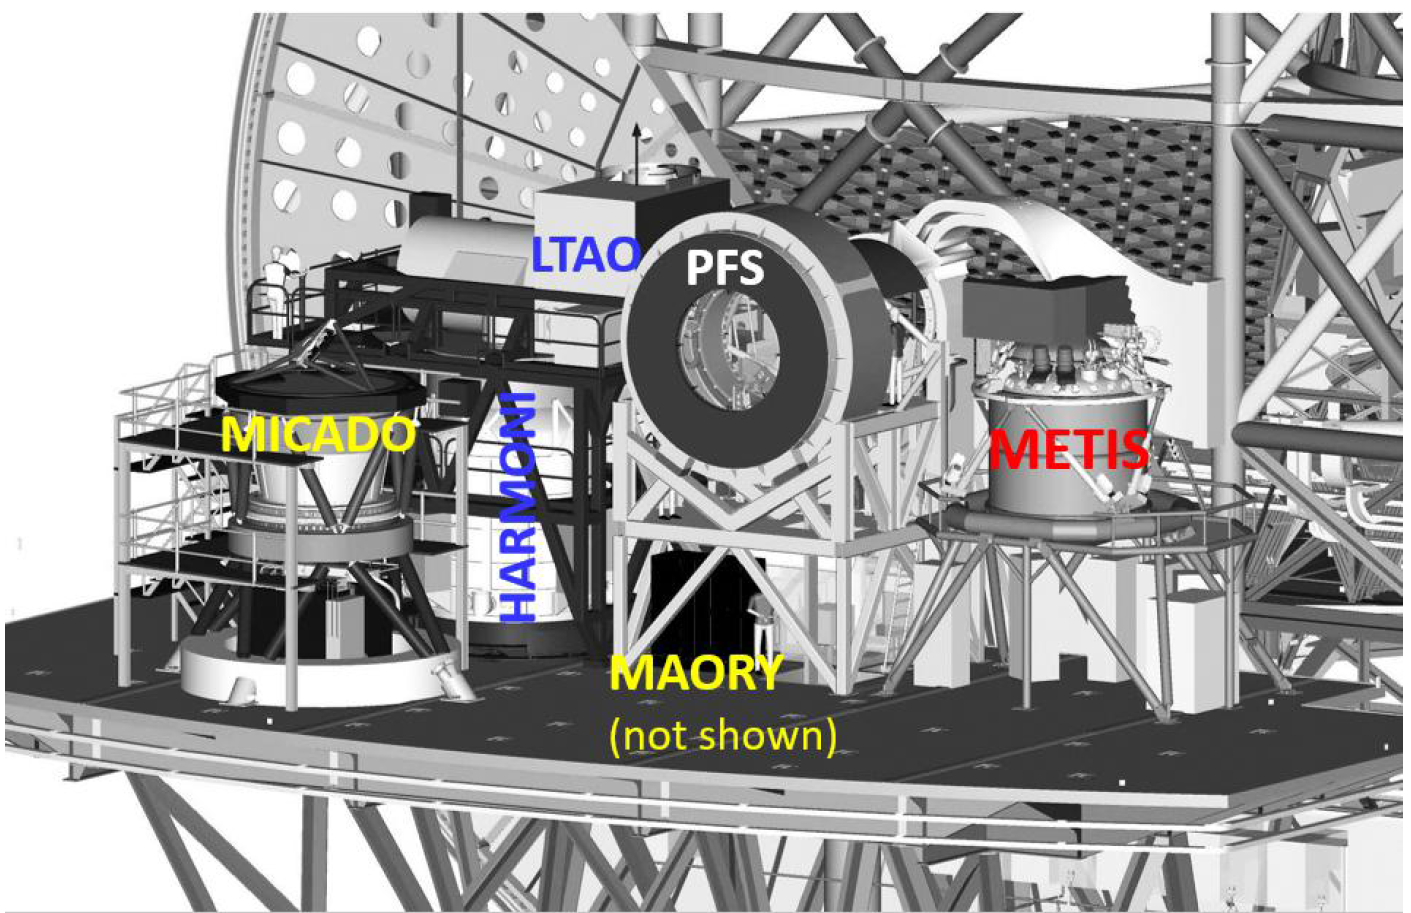
\includegraphics[width=12 cm]{Figures/ELT_nas_deck.png}
\caption{View of the Instruments on ELT's Nasmyth platform.  Things to note are the PFS and METIS on the right.  The SLAO
system needs fit in between the PFS and METIS. \cite{METISupdate}}
\label{fig:ELT_nas_deck}
\end{figure}

The structure of the SLAO system needs to fit in between the Pre-focal station and
METIS itself.  Therefore, the more compact the structure is, the better.  One of the
main constraints is the width of the structure.  This is dominated by the laser
pick-off mirror.  METIS, as previously discussed in Chapter \ref{Chapter2}, is a
mid-infrared instrument.  Because the SLAO system would be outside of the cyrostat,
a beam-splitter would radiate too much in the infrared.  This would be a large
source of noise and would not be an ideal solution.  An ideal solutions was
researched in Benjamin's report of an Annular Mirror \cite{arcier}.  This would take
advantage of the central obscuration (ELT M2) as well as the fact that the observed
object and the laser spot are a different distance from the primary mirror.  From
this, dimensions for an annular mirror were made to pickup laser light while
allowing the science image to pass through (Figure \ref{fig:ann_mirror}).


\begin{figure}[h!]
\centering
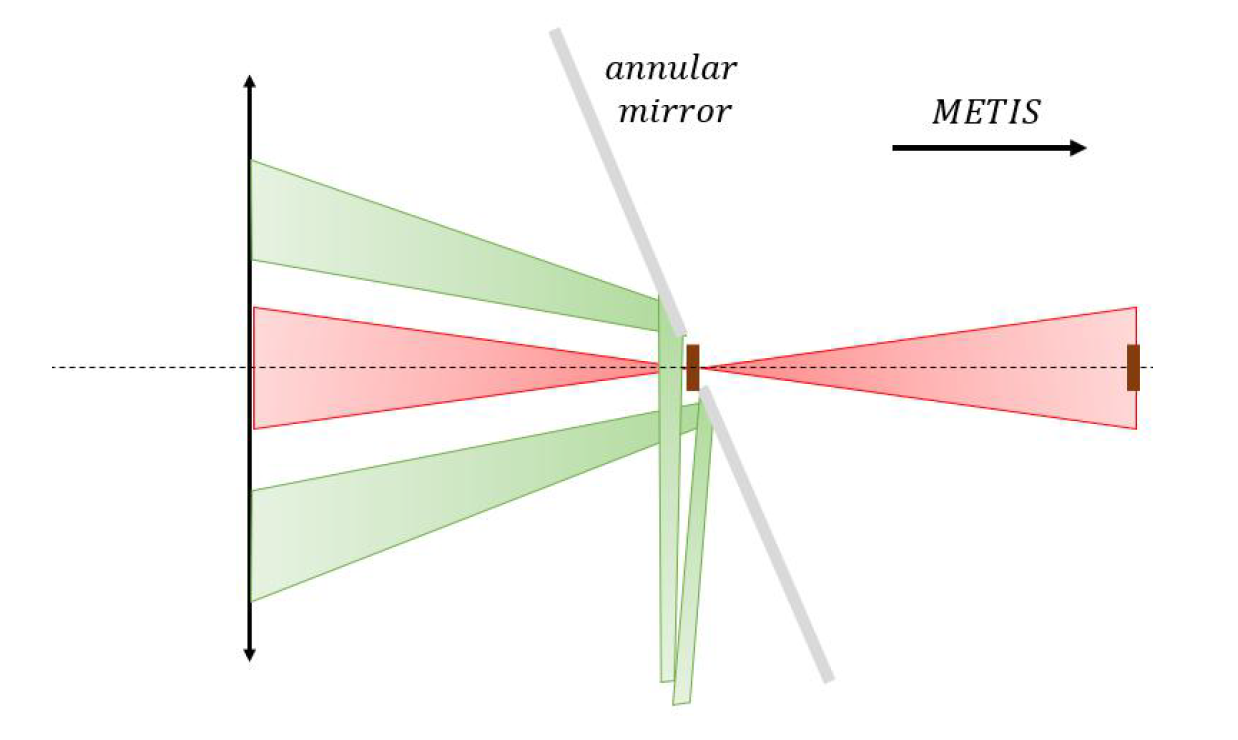
\includegraphics[width=12 cm]{Figures/ann_mirror.png}
\caption{A representation of the Annular mirror design.  The green object represents the laser light and the red represents light from infinity. \cite{arcier}}
\label{fig:ann_mirror}
\end{figure}

This puts a pretty tight tolerance on where the annular pick-off mirror can be
placed.  This will covered in finer detail in Chapter \ref{Chapter3}.  What this
means for the opto-mechanical design is that the diameter of the annular mirror
drives the width dimension.  The radius calculated by ZEMAX of the mirror is 240mm,
which gives a width of $2 \times r \times \cos(45) \approx 340$mm.  From there,
light converges and the optics get smaller.  To make the SLAO system more compact,
we implemented fold mirrors to angle the light.

\section{Mechanical Components}
\label{sec:mech_comp}

With the light path folded into a manageable profile, the next task was to design a
cage around the optics.  The cage supports were taken from the manufacturer ITEM. 
The selected profile was chosen due to it having the least amount of sag for the
weight of the largest optic \cite{item}.  From this profile, the cage was designed
to have a total dimension of $1.2m \times 1.2m \times 400mm$.  The profile of the
support structure can be seen in Figure \ref{fig:item}.  


\begin{figure}[h!]
\centering
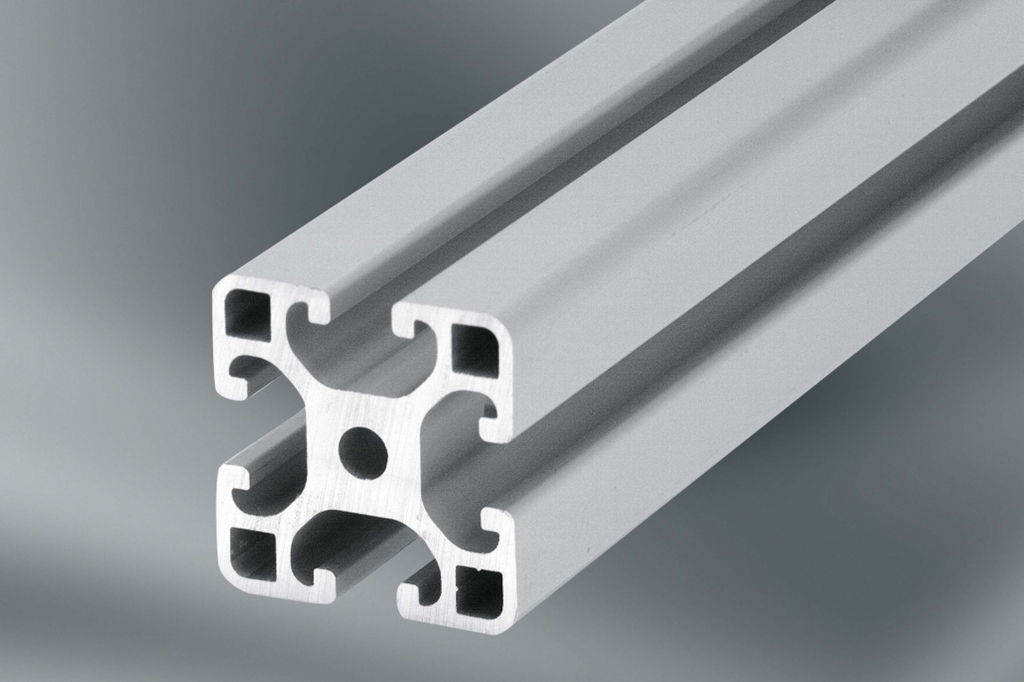
\includegraphics[width=10 cm]{Figures/item_profile.jpg}
\caption{Profile of the cage support structure.  Made by ITEM. \cite{item}}
\label{fig:item}
\end{figure}


Next, the design called for two moving stages.  One for the annular mirror to move
out of the light path for SCAO observations, the other for the altitude compensator
stage.  Benjamin Arcier's optical design had a range of travel equal to 182.178$mm$.  Therefore,
a stage that could handle both moving the annular mirror out of the way as well as
for altitude correction would be ideal.  The Thorlabs 220mm translation stage was % Reference Altitude correction in the later section.
chosen.  The stage had the range of travel needed for both moving stages and had a
desirable accuracy for the altitude correction.  I will go further into altitude correction
in Section \ref{optical_constraints}.  Though the horizontal loads limit
is quite low, this will not be a problem since all moving stages were placed to move
normal to gravity.  The translation stage also had a small breadboard attached to it
for mounting optics as seen in Figure \ref{fig:thor}.  More specifications on the
translation stage can be found in Table \ref{tab:thor}.


\begin{figure}[h!]
\centering
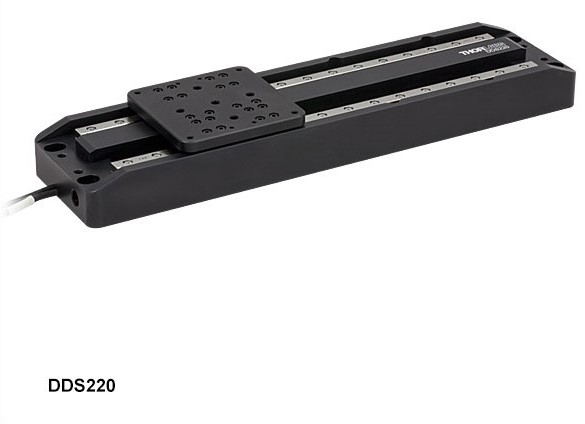
\includegraphics[width=9 cm]{Figures/thor.jpg}
\caption{Thorlabs translation stage \cite{thor}}
\label{fig:thor}
\end{figure}


\begin{table}[h!]
\begin{tabular}{|l|c|}
\hline
\textbf{Travel Range}                        & $220mm$                  \\ \hline
\textbf{Max Velocity}                        & $300mm/s$                \\ \hline
\textbf{Min Achievable Incremental Movement} & $0.1 \mu m$              \\ \hline
\textbf{Bidirectional Repeatability}         & $\pm 0.25 \mu m$         \\ \hline
\textbf{Horizontal Load Capacity (Max)}      & $3.0 kg$                 \\ \hline
\textbf{Actuator Type}                       & Brushless DC Servo Motor \\ \hline
\textbf{Cable Length}                        & $2.7m$                   \\ \hline
\end{tabular}
\caption{Spec table for the Thorlabs 220mm translation stage. \cite{thor}}
\label{tab:thor}
\end{table}

With these components, a high-order cage system was designed for the optical design.
Although the optical design had less than desirable characteristics, we
could prove that a SLAO system could fit into the space envelope between METIS and
the PFS of ELT.  The next step would be to find a more cost effective optical design
to demonstrate to ESO that a more cost effective alternative to a LTAO system is
feasible.  


% \begin{figure}[ht!]
% \centering
% 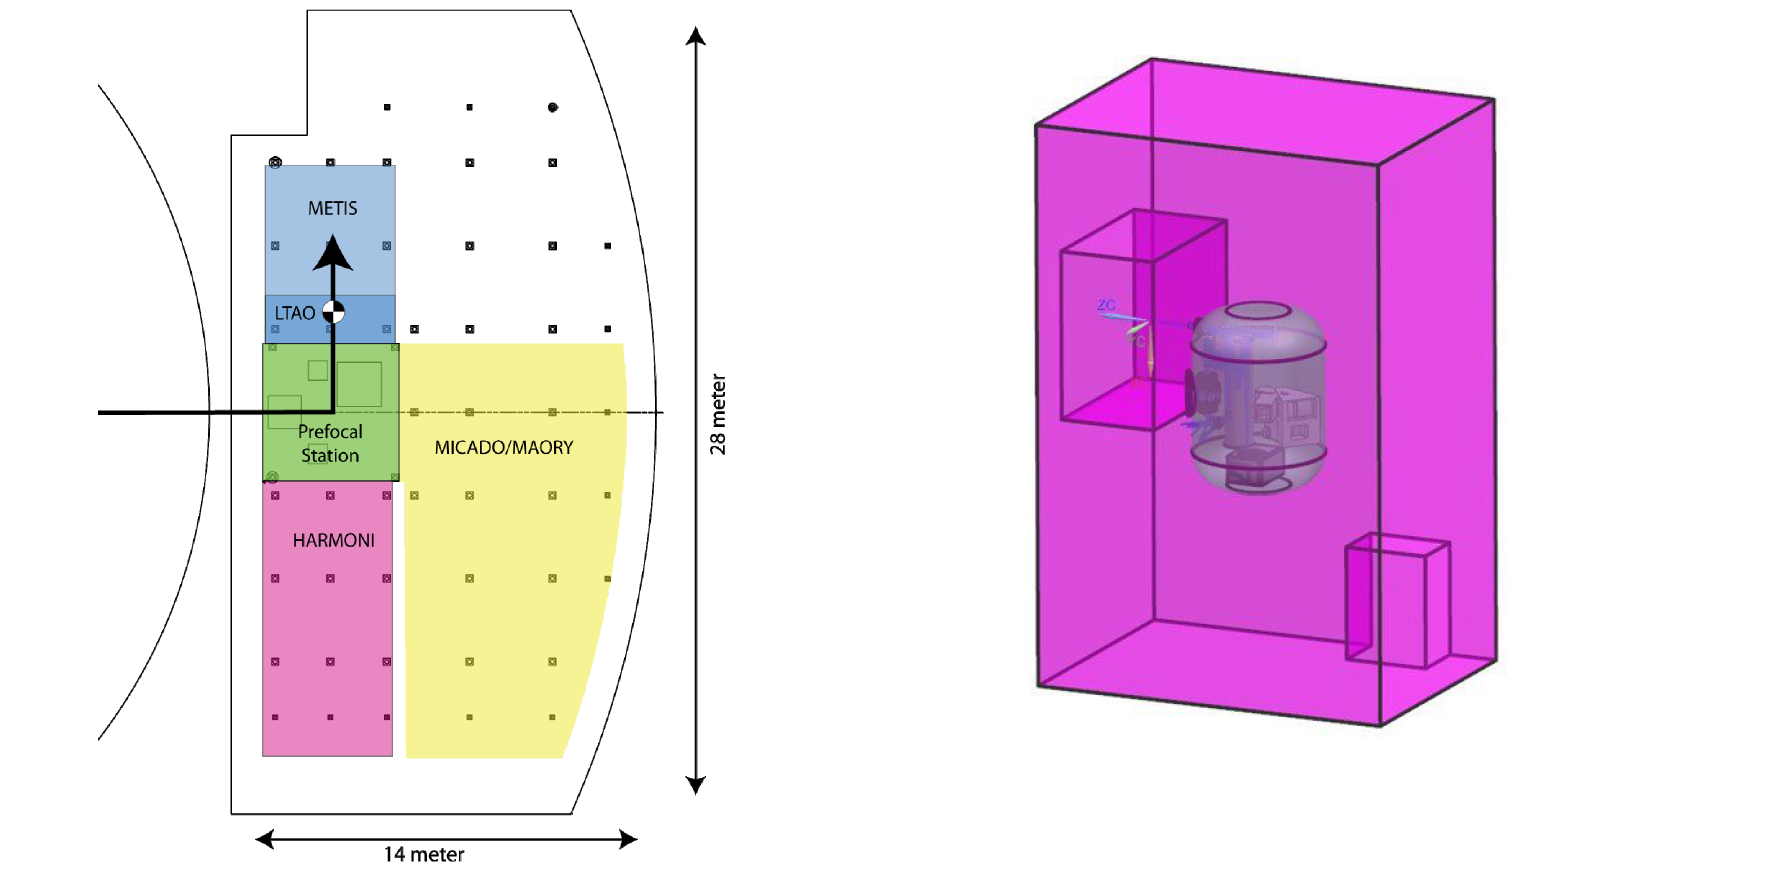
\includegraphics[width=14 cm]{Figures/METIS_platform.png}
% \caption{(Left) The layout for the ELT Nasmyth A Platform.  (Right) MEITS cyrostat within the allotted volume.  \cite{METISSPIE2016}}
% \label{fig:metis_phys}
% \end{figure}

% \begin{figure}[H]
% \centering
% \begin{subfigure}{.5\textwidth}
%   \centering
%   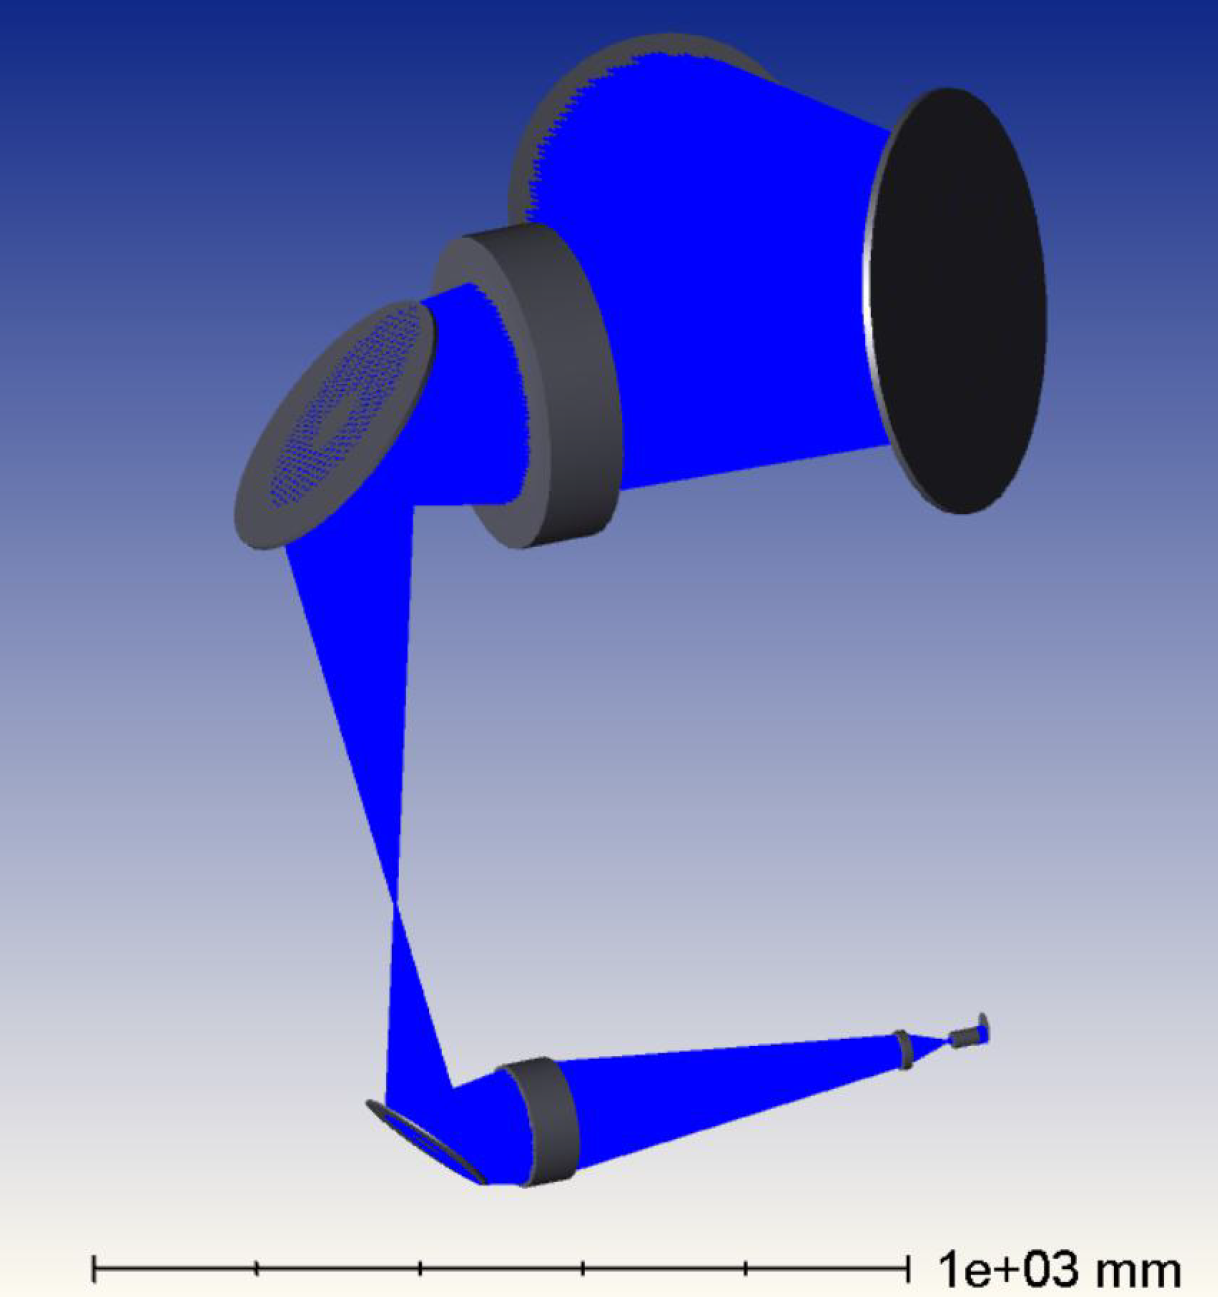
\includegraphics[width=6cm]{Figures/Ben_optic_design.png}
%   \caption{A shaded model of Benjamin's optical design.  Light comes from the top right and folds down to a camera on the bottom right}
%   \label{fig:ben_optic}
% \end{subfigure}%
% \begin{subfigure}{.5\textwidth}
%   \centering
%   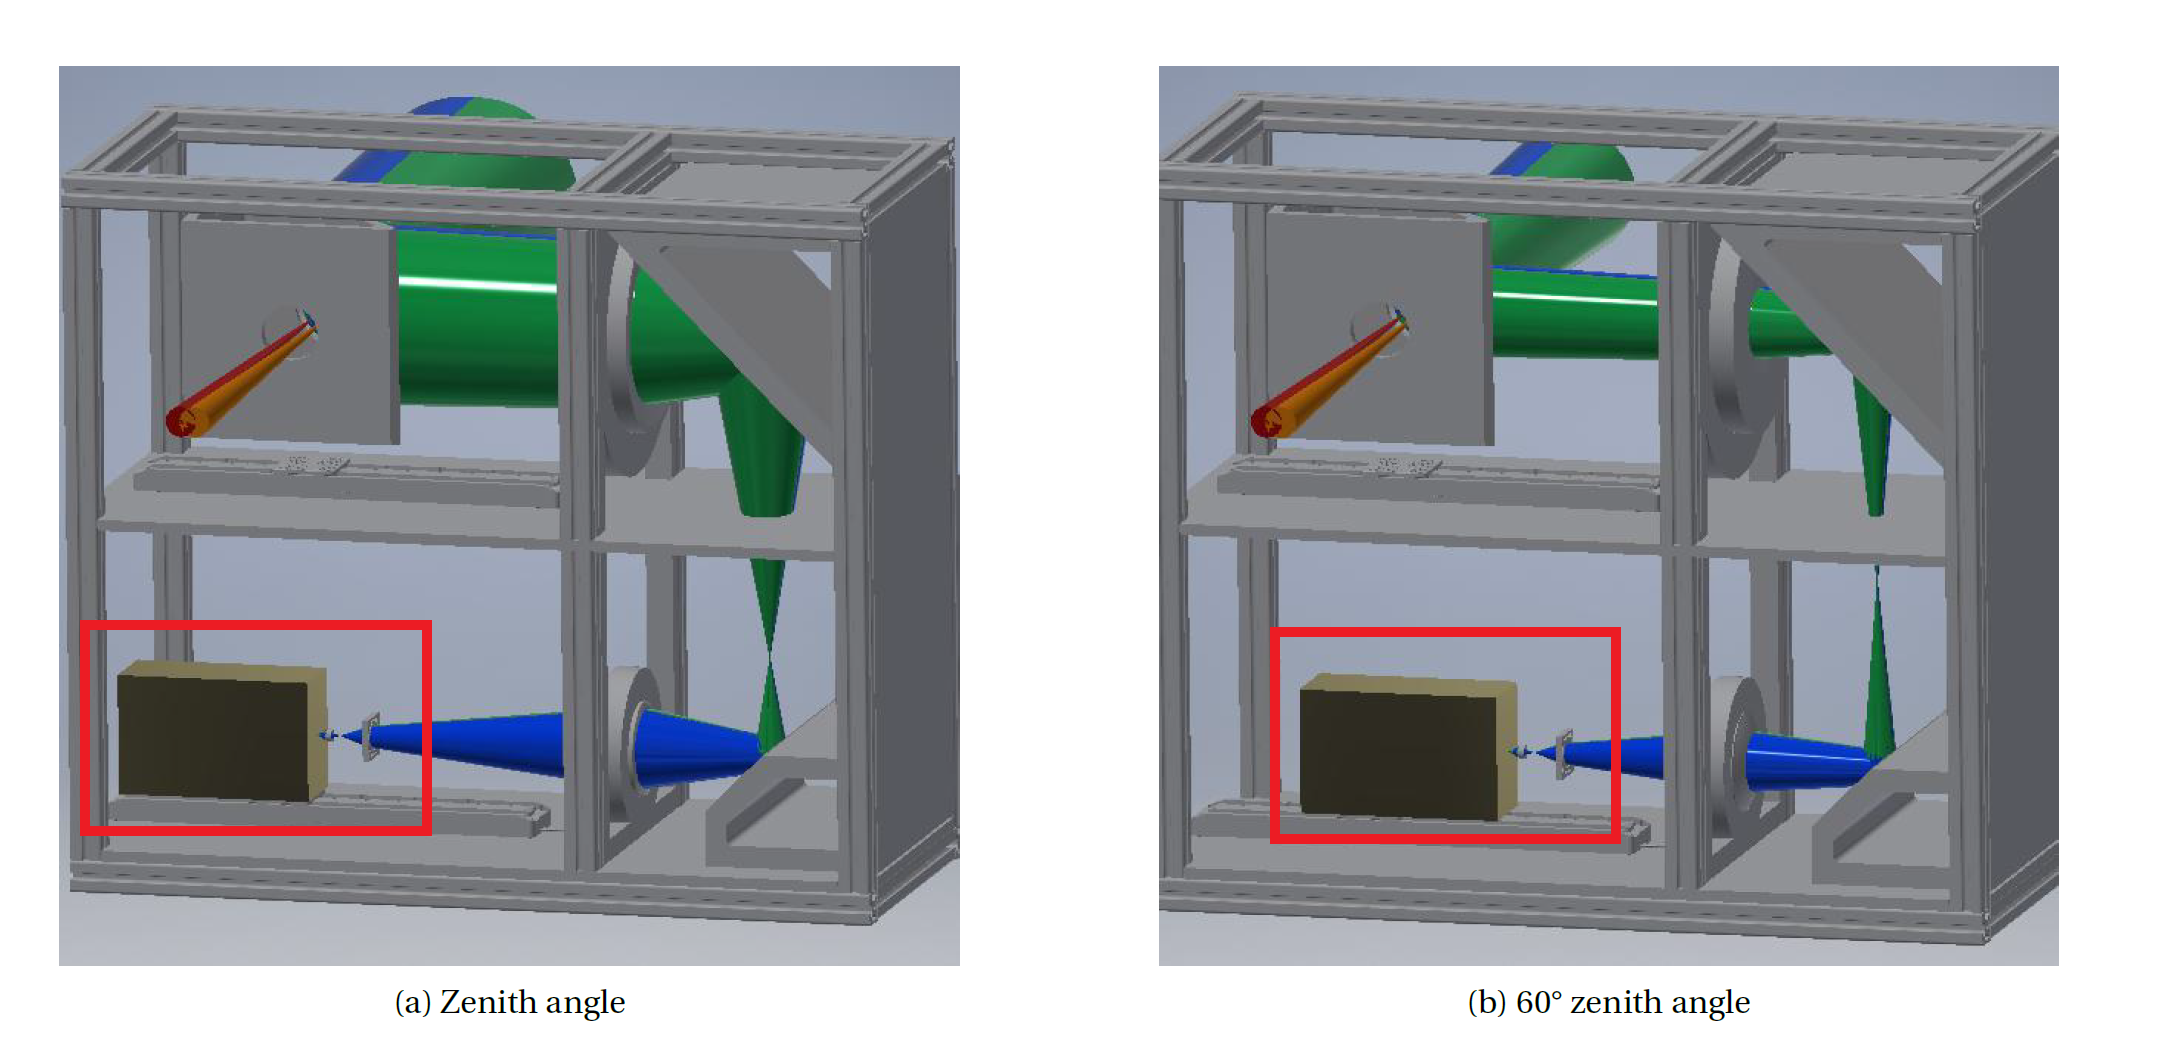
\includegraphics[width=8cm]{Figures/camera_change.png}
%   \caption{A figure showing how the original design compensated for the change in focus.  All objects in the red square were on a moving stage}
%   \label{fig:camera_change}
% \end{subfigure}
% \caption{Figure showing the end result of Benjamin Arcier's research.\cite{arcier}}
% \label{fig:pickup}
% \end{figure}